%#! platex %f && dvipdfmx -d 5 sampleslide161018
%
%
% このファイルは,ほぼミニマム仕様です.
% 詳しい使い方は,マニュアルを読むか 「latex beamer」などで検索して調べてください.
%
% latex sampleslide161018.tex
% dvipdfmx sampleslide161018.dvi
% これで  sampleslide161018.pdf が作成されるはずです.
%
% もし yatex をインストールしていると,emacs 上から,Ctr-x t j で pdf ファイルが作成できます. 
%
\documentclass[14pt,dvipdfmx]{beamer}
\AtBeginDvi{\special{pdf:tounicode EUC-UCS2}} % 「しおり」の文字化け防止用
%
% 一つ選ぶ
%\usetheme{AnnArbor}
%\usetheme{Berlin}
%\usetheme{Copenhagen}
%\usetheme{Malmoe}
%\usetheme{Madrid}
%\usetheme{Darmstadt}
\usetheme{Pittsburgh}

\usefonttheme{professionalfonts}  

\usepackage{bm}
\usepackage{graphicx}
\usepackage{amsmath}
\usepackage{amssymb}
\usepackage{latexsym}
\usepackage{alltt}

\renewcommand{\familydefault}{\sfdefault}
\renewcommand{\kanjifamilydefault}{\gtdefault}

\setbeamerfont{title}{size=\large,series=\bfseries}
\setbeamerfont{frametitle}{size=\large,series=\bfseries}
\setbeamerfont{footline}{size=\small,series=\bfseries}

\setbeamertemplate{frametitle}[default][center]
\setbeamertemplate{blocks}[rounded]
\setbeamertemplate{navigation symbols}{}
\setbeamertemplate{footline}[page number]

\setbeamercolor{footline}{fg=black,bg=black}

\bmdefine{\bx}{x}
\bmdefine{\bX}{X}
\bmdefine{\by}{y}

\title{脳とコンピュータ}
\author{伊達 章}
\institute{宮崎大学}
\date{2016年10月18日}

%\title[Short title]{タイトル}   % Short title は省略可。ヘッダ、フッタの表示で利用
%\subtitle{副題}                 % 省略可
%\author[著者略称]{氏名}
%\institute[所属略称]{所属}


\begin{document}

\frame{\titlepage}

\section{発表の概要}

\begin{frame}[c]

  \frametitle{講義のテーマ}
  
  \begin{itemize}
  \item<1-> 脳は情報処理をする素晴らしい装置{\color{red}!}
  \item<2-> コンピュータと脳の比較

特に情報表現と計算の観点から

  \item<3-> 神経回路モデルのダイナミックス
  \item<4-> 自己組織化とは
  \item<5-> 情報数理科学による{\color{blue}脳の情報原理}の理解
  \end{itemize}

\end{frame}

\section{脳とコンピュータ}
\subsection{問題提起}

\begin{frame}
  \frametitle{}
  \begin{center}\large\bfseries
   脳はコンピュータか?

\pause

   \Huge  \color{red}Yes!
  \end{center}
\end{frame}


\subsection{コンピュータとは}

\begin{frame}[plain]

  \begin{center}\Huge\bfseries
   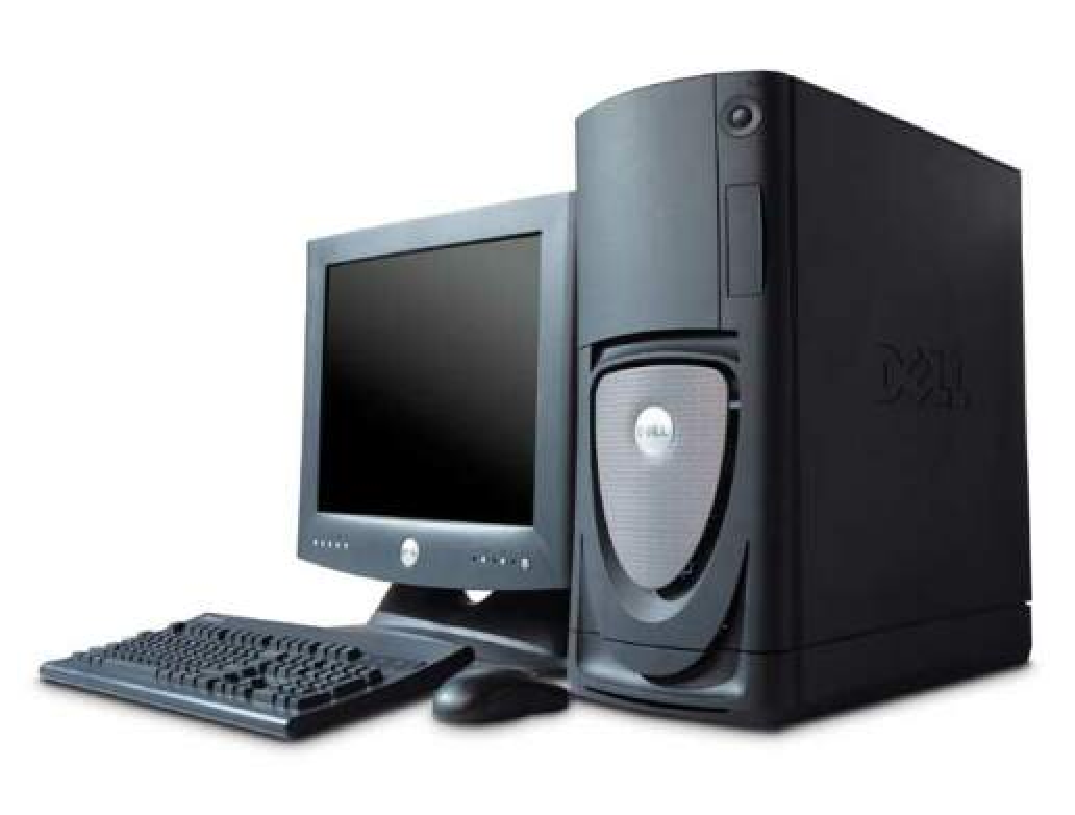
\includegraphics[width=.8\linewidth]{computer.eps}\\
   \color{blue}コンピュータ
  \end{center}

\end{frame}

\subsection{脳とコンピュータ}

\begin{frame}

  \frametitle{脳とコンピュータ}
\centering
\includegraphics[width=.48\linewidth]{advnn001.eps}
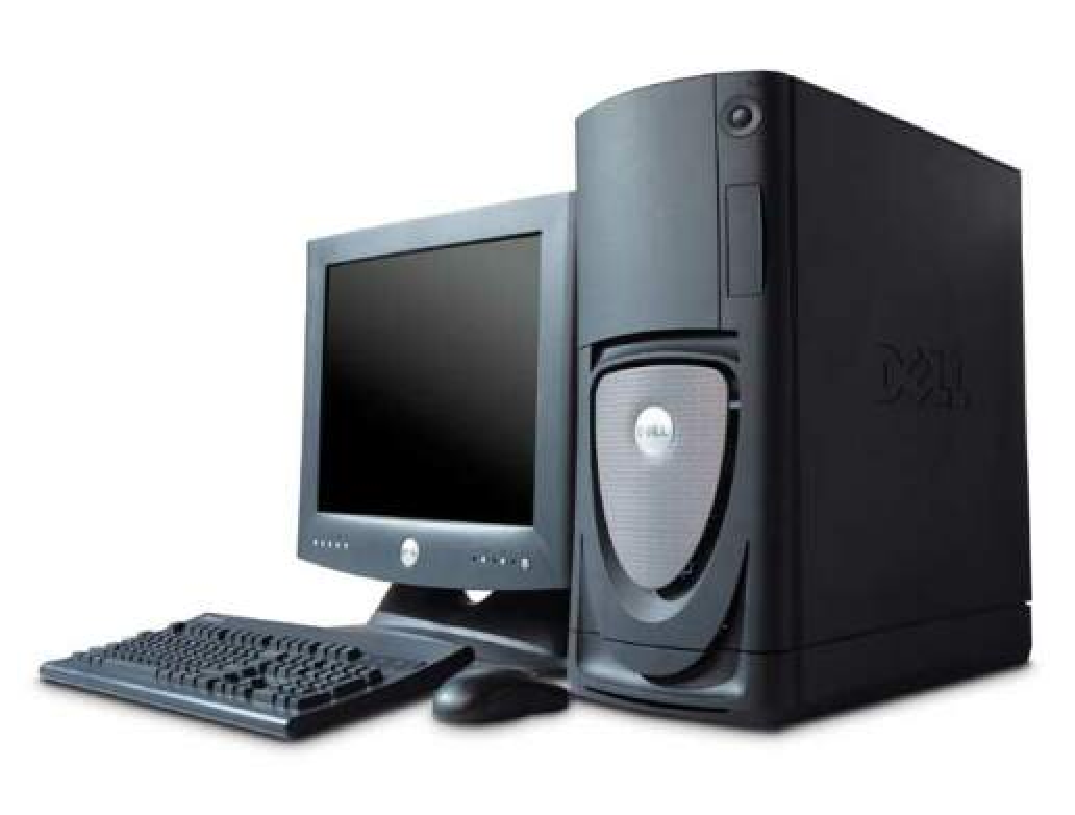
\includegraphics[width=.48\linewidth]{computer.eps}

\end{frame}


\subsection{神経細胞のモデル}

\begin{frame}

  \frametitle{神経細胞のモデル}
$$
x_i = {\rm sgn} \sum_{j=1}^{n} w_{ij} x_j -h
$$
ここで,$h$ はしきい値.

\end{frame}

\subsection{確率の基礎}

\begin{frame}
  \frametitle{同時確率,周辺確率}

\begin{eqnarray}
\bx & = & (x_1,x_2, \cdots, x_n)^{\rm T} \\
p(\bx) & = & \Pr ( \bX = \bx ) = \Pr ( X_1=x_1, \cdots, ) \\
p(y_i | x_i) & = & \frac{1}{\sqrt{2\pi} \sigma } {\rm e}^{-\frac{(y_i - x_i)^2}{2\sigma^2}}\\
p(\bx,y) & = & 0.3 
%\Pr (x,y) & 
\end{eqnarray}

\begin{center}
{\small 
\begin{tabular}{|c|c|c|c|} \hline
& $B_1$ (風邪) & $B_2$ (風邪なし) & $p(A_i)$ \\ \hline
$A_1$ (熱あり)& 0.55 & 0.05 & 0.60  \\
$A_2$ (熱なし)& 0.10 & 0.30 & 0.40 \\ \hline
$p(B_j)$ & 0.65 & 0.35 & \\ \hline
\end{tabular}
}
\end{center}

\end{frame}


\begin{frame}

\frametitle{脳の特性}

\begin{columns}[c]

\column{60mm}

 \begin{itemize}

\item 総合能力は抜群

\item 正確な計算は苦手

\item 忘却機能に優れている

 \end{itemize}

\column{60mm}

%\framebox{\includegraphics[width=1.5in]{./advnn001.eps}}
\includegraphics[width=\textwidth]{./advnn001.eps} 

\end{columns}

\end{frame}


\end{document}